%!TEX root = ../dissertation.tex
\chapter{Valutazione retrospettiva}
\label{conclusion}
Il seguente capitolo espone il bilancio complessivo dell’esperienza di stage, valutando il raggiungimento degli obiettivi posti dal Piano di Lavoro e presentando le conoscenze acquisite durante questo periodo.

\section{Conseguimento degli obiettivi}
Gli obiettivi individuati durante la stesura del Piano di Lavoro sono stati ripartiti in tre tipologie e possono essere riassunti nel seguente modo:
\begin{itemize}
    \item Obbligatori
        \begin{itemize}
            \item  Studio dell’intero sistema Beryllium;
            \item Comprensione del mondo SAM, SPLA e del prodotti Microsoft di interesse;
            \item Configurazione dell’ambiente di test per il prodotto Microsoft Dynamic CRM;
            \item Progettazione, sviluppo e test di un prototipo della componente "Microsoft Dynamic CRM
            feature for Beryllium Data Collector" per l’ultima versione di Microsoft Dynamic CRM;
            \item Documentazione di progetto.
        \end{itemize}
    \item Desiderabili
        \begin{itemize}
            \item Completa integrazione con la componente Beryllium Data Collector.
        \end{itemize}
    \item Facoltativi
        \begin{itemize}
            \item  Sviluppo e test della componente "Microsoft Dynamic CRM feature for Beryllium Data Collector" per almeno una versione più vecchia di Microsoft Dynamic CRM;
            \item F02: Sviluppo e test della componente "Microsoft Dynamic CRM feature for Beryllium Data
            Collector" per almeno due versioni più vecchie di Microsoft Dynamic CRM.
        \end{itemize}
\end{itemize}
L'esecuzione dei test di unità e di integrazione, hanno permesso di verificare il corretto funzionamento di tutte le componenti del \emph{software}, mentre i test di sistema
sono stati necessari al fine di capire quali dei requisiti definiti durante l'analisi erano stati implementati.
Grazie all'esecuzione e al tracciamento di tali requisiti
è stato possibile determinare gli obiettivi raggiunti al termine dello stage.
\\
Come si può evincere dal grafico successivo, sono stati raggiunti gli obiettivi obbligatori e desiderabili, mentre quelli facoltativi, per mancanza di tempo, non sono stati finalizzati.
\begin{figure}[H]
\centering
\captionsetup{justification=centering,margin=2cm}
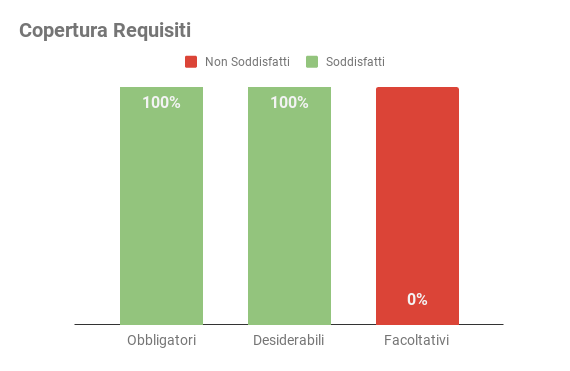
\includegraphics[width=0.8\textwidth ]{figures/copertura.png}
\caption [Grafico copertura dei requisiti raggiunta]{Copertura dei requisiti raggiunta alla fine dello stage \label{fig:coperturarequisiti}}
\end{figure}
\section{Conoscenze preliminari}
Il corso di laurea triennale in Informatica fornisce solide conoscenze di base di carattere tecnico e allo stesso tempo
si occupa si far apprendere agli studenti i meccanismi fondamentali della materia e di stimolare flessibilità di pensiero e la capacità di \emph{problem solving}.
Personalmente, attraverso lo stage, ho avuto la possibilità di mettere in pratica le conoscenze e gli strumenti ricevute dagli insegnamenti dei corsi di Ingegneria del Software, Programmazione ad Oggetti e Basi di Dati. \\
Dunque, per quanto concerne il processo di sviluppo del progetto a cui mi sono dedicata, le conoscenze preliminari sono risultate sufficientemente adeguate. 
Invece, rispetto alle esigenze del contesto aziendale in cui sono stata inserita, ho riscontrato delle difficoltà iniziali riguardo alla gestione dei sistemi informativi e della loro sicurezza, causate da una scarsa preparazione accademica di tali argomenti.
\section{Conoscenze acquisite}
Il processo di sviluppo del progetto di stage ha richiesto lo studio e la successiva applicazione di tecnologie mai affrontate in passato.
Il prodotto \emph{Microsoft Dynamics} CRM, sul quale si basava il progetto formativo, mi ha permesso di ottenere una visione consapevole riguardo al mondo dei \emph{software} e del \emph{licensing} Microsoft. 
Inoltre ho rafforzato le mie conoscenze sulla gestione di un ambiente Windows dal lato \emph{server} e ho avuto la possibilità di apprendere il linguaggio C\# e di sfruttare concretamente le potenzialità di PowerShell.
In particolare ho conseguito le seguenti conoscenze:
\begin{itemize}
    \item \emph{Visual Studio 2016 Community}: è stato l’ambiente di sviluppo utilizzato per il progetto. Le diverse funzionalità offerte dall’IDE si sono rivelate particolarmente utili lavorando in ambiente Microsoft e la vasta documentazione fornita da \gl{MSDN} ha permesso di velocizzare in modo significativo il suo apprendimento;
    \item \emph{Windows Server 2012 R2}: durante il processo di sviluppo è stato essenziale apprendere le funzionalità di base della gestione dei \emph{server} Microsoft;
    \item C\#: lo sviluppo della \emph{feature} ha richiesto l’utilizzo di C\# come linguaggio principale.
    Grazie alla ricca documentazione ufficiale la fase di codifica si è svolta agevolmente;
    \item \emph{Powershell}: il linguaggio  permette un accesso estremamente semplice ad una vasta quantità di funzionalità per interfacciarsi con i prodotti Microsoft e ciò ha permesso di estrarre dati utili in fase di test;
    \item \emph{Active Directory}: imparare il funzionamento di questo framework si è rivelato fondamentale per l’utilizzo di \emph{Microsoft Dynamics} CRM 2016, il quale si integrava con il dominio aziendale e perciò è stato necessario apprendere come gestirlo;
    \item \emph{Microsoft Dynamics} CRM 2016: al fine di sviluppare la relativa \emph{feature} è stato necessario installare e configurare sul \emph{server} il prodotto. Inoltre, ho popolato le diverse tabelle con vari tipi di record, il che ha richiesto uno studio abbastanza approfondito del
    funzionamento di questa tecnologia;
    \item SAM e SPLA: durante il corso del progetto è stato necessario interagire più volte con il reparto SAM per apprendere le diverse regole di \emph{licensing} dei prodotti Microsoft in SPLA, che mi ha permesso di ottenere una visione generale di questi concetti mai approfonditi durante il corso universitario.
\end{itemize}